\documentclass[a4paper]{article}

\usepackage{fullpage}               % Reduce white space around margins
\usepackage{graphicx}               % For including images
\usepackage{chngcntr}               % For section-wise table/figure counters
\usepackage{caption}                % For specifying figure/table captions and its attributes
\usepackage{geometry}               % For specifying margin sizes
\usepackage{amssymb}                % For simple math symbols
\usepackage{verbatimbox}            % For a neat box around verbatim text
\usepackage{multirow,tabularx}      % For row splits in a table

\date{}                             % Don't print the date
\linespread{1.5}                    % Line spacing = 1.5
\counterwithin{table}{section}      % Count tables per-section
\counterwithin{figure}{section}     % Count figures per-section
\geometry{a4paper, margin=0.82in}

\begin{document}

% Create title page
    \begin{titlepage}
        \vspace*{\fill}
        \begin{center}
            {\huge \bf ECE 521 - Computer Design Techniques \\ Fall 2014 \\ \vspace {8 mm} \\ \LARGE \bf Cache and Memory Hierarchy Design \\ \vspace{4 mm} Project Report}
            
            {\vspace{9 mm} \it \large Prepared by \\ \bf \Large Aravindhan Dhanasekaran\\ \bf \large adhanas@ncsu.edu}
        \end{center}
        \vspace*{\fill}
    \end{titlepage}


\newpage
\tableofcontents
\listoffigures
\listoftables
\newpage


\section{Introduction}
In this project, a simulator for cache hierarchy has been built which can simulate three levels of caches: primary L1 cache (complemented by victim cache) and secondary L2 cache. This project report analyzes the various cache configurations, explains the trends observed in the different configurations in terms of miss rate and average access time and suggests a cache configuration that works best with the given set of inputs. The simulator supports different replacement algorithms (least recently used and least frequently used) and write reference handling (write back/write allocate and write through/no write allocate) for the primary cache, but to keep the results comparable, all the caches use LRU and wrie back/write allocate policies.


\section{Formulas}
Some of the important formulas that are used to characterize cache performance are briefly discussed in this section.

\subsection{Memory Address to Cache Line Conversion}
The address generated by the processor refers to the physical (or virtual) address where the data or instruction is stored. In order to perform a cache look-up on the CPU generated address, the memory reference must be converted into appropriate cache line. This will be different for different caches based on cache attributes such as cache size, block size and cache set associativity and so on.

\[32BitAddress = <tags, index, blockOffset>\]

\[blockOffset = \log_2 (blockSize)\]

\[index = \log_2 (numSets)\]
\[numSets = \frac{cacheSize}{blockSize * setAssoc}\]

\[tags = 32 - index - blockOffset\]

\subsection{Cache Miss Rate}
Cache miss rate denotes the ratio of number of cache misses to the total number of references. The lower the cache rate, the better is the cache performance. Cache miss rate is one of the important attribute of a cache which helps in understanding the characteristics of the cache. All cache performance improvement  methods would decrease the cache miss rate in one way or the other.

\[cacheMissRate = \frac{(numReadMisses + numWriteMisses)}{(numReads + numWrites)}\]

\subsection{Average Access Time}
Average Access Time (AAT) denotes the time average time required to process a request. It encompasses the time spent on cache look-ups, fetching data from memory on cache misses and writing back the dirty block in case of dirty block eviction. AAT can be used to guage the performance of a cache in an informal way. 

\[AAT = \frac{totalAccessTime}{(numReads + numWrites)}\]
\[totalAccessTime = ((numReads + numWites) * cacheHitTime) +\]
                             \[(numReadMisses + numWriteMisses) * missPenalty)\]


\section{Cache Simulator}
As a part of this project, a cache simulator has been designed. The simulator is capable of simulating L1 cache, L1 cache with victim cache, L1 cache \& L2 cache and L1 cache with victim cache \& L2 cache. The input to the simulator is an ASCII file with memory references and reference type - read or write (simulates CPU memory requests). The cache attributes such as block size, L1 cache size, L1 cache set associativity, victim cache size, L2 cache size and L2 cache set associativity during run time.

\begin{verbatim}
$ ./sim_cache 
Usage: ./sim_cache <block-size> <l1-cache-size> <l1-set-assoc> <victim-cache-size>
                   <l2-cache-size> <l2-set-assoc> <trace-file>
    block-size          : size of each cache block in bytes; must be a power of 2.
    l1-cache-size       : size of the L1 cache in bytes.
    l1-set-assoc        : set associativity of the L1 cache.
    victim-cache-size   : size of the victim cache in bytes; 0 disables victim cache.
    l2-cache-size       : size of the L2 cache in bytes; 0 disables L2 cache.
    l2-set-assoc        : set associativity of the L2 cache.
    trace-file          : CPU memory access file with full path.

\end{verbatim}

\begin{verbatim}
    $ head -n 9 gcc_trace.txt 
    w 400341a0
    r dfcfa8
    w 7b034dd4
    r df7c48
    r 7b034dd4
    r 423aebbc
    r 423aebb8
    r 423aebbc
    r 40002634
\end{verbatim}


\section{Experiments}
Various experiments with different cache configurations and different memory trace files were run in order to understand the cache performance affecting attributes. This section represents the different runs, the cache parameters of every run and the cache statistics in tables and in graphs. The data will be analyzed in following section.

In all the following experiments, four different memory trace files are used: gcc\_trace, go\_trrace, perl\_trace and vortex\_trace.

\subsection{L1 Cache: Size, Set Associativity and Miss Rate}
In this experiment, only L1 cache is used (victim and L2 caches are disabled). The purpose of the experiment is to study the relationship between the size of the cache and miss rate. The cache configuration is given in Table \ref{tab:l1mr_config}. All four traces were run with varying L1 cache sizes and varying cache associativity. The results are tabulated in Tables \ref{tab:l1mr_data_sa1}, \ref{tab:l1mr_data_sa2}, \ref{tab:l1mr_data_sa4}, \ref{tab:l1mr_data_sa8} and the same is plotted as graphs in Figures \ref{fig:l1mr_graph_sa1}, \ref{fig:l1mr_graph_sa2}, \ref{fig:l1mr_graph_sa4}, \ref{fig:l2mr_graph_sa8}.

\begin{table}[htbp]
    \centering
    \begin{center}
        \begin{tabular}{|l|l|}
            \hline
            \bf Cache Attributes & \bf Value \\ \hline
            Block size &  32 \\
            L1 cache size & Variable \\
            L1 cache SA & Variable \\
            Victim cache size & Disabled \\
            L2 cache size & Disabled \\
            L2 cache SA & Disabled \\
            \hline
        \end{tabular}
        \captionsetup{justification=centering}
        \caption{Cache Configuration for L1 Cache Size vs. Miss Rate Experiment}
        \label{tab:l1mr_config}
    \end{center}
\end{table}

\begin{table}[htbp]
    \centering
    \begin{tabular}{|c|c|c|c|c|c|c|c|c|}
        \hline
        \multirow{2}[4]{*}{\bf L1 Cache Size} & \multicolumn{2}{c|}{\bf gcc} & \multicolumn{2}{c|}{\bf go} & \multicolumn{2}{c|}{\bf perl}          &\multicolumn{2}{c|}{\bf vortex}\\
        \cline{2-9} & \bf MR & \bf AAT & \bf MR & \bf AAT & \bf MR & \bf AAT & \bf MR & \bf AAT \\
        \hline
        128 & 0.4332 & 9.4232 & 0.4518 & 9.8145 & 0.5744 & 12.3889 & 0.5113 & 11.0621 \\
        256 & 0.3336 & 7.3312 & 0.3438 & 7.5458 & 0.4883 & 10.5779 & 0.3817 & 8.3419 \\
        512 & 0.2653 & 5.8994 & 0.2792 & 6.1906 & 0.3670 & 8.0349 & 0.2858 & 6.3292 \\
        1024 & 0.1935 & 4.3925 & 0.2424 & 5.4192 & 0.2801 & 6.2116 & 0.1601  & 3.6924 \\
        2048 & 0.1477 & 3.3473 & 0.0904 & 2.2336 & 0.1929 & 4.3852 & 0.1101 & 2.6475 \\
        4096 & 0.1002 & 2.4481 & 0.0737 & 1.8933 & 0.1108 & 2.6718 & 0.0707 & 1.8294 \\
        8192 & 0.0670 & 1.7711 & 0.0631 & 1.6902 & 0.0675 & 1.7811 & 0.0468 & 1.3464 \\
        16384 & 0.0461 & 1.3710& 0.0607 & 1.6770& 0.0492 & 1.4367 & 0.0338 & 1.1131 \\
        \hline
    \end{tabular}
    \captionsetup{justification=centering}
    \caption{Experiment Data for L1 Cache Set Associativity = 1}
    \label{tab:l1mr_data_sa1}
\end{table}

\begin{figure}
    \centering
    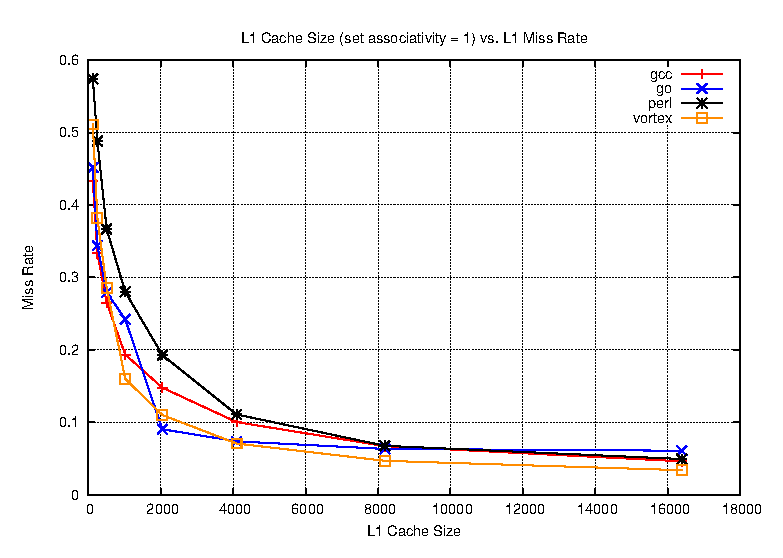
\includegraphics[scale=1.32] {l1_sa_1.eps}
    \captionsetup{justification=centering}
    \caption{L1 Cache Size vs. L1 Miss Rate for L1 Set Associativity = 1}
    \label{fig:l1mr_graph_sa1}
\end{figure}

\begin{table}[htbp]
    \centering
    \begin{tabular}{|c|c|c|c|c|c|c|c|c|}
        \hline
        \multirow{2}[4]{*}{\bf L1 Cache Size} & \multicolumn{2}{c|}{\bf gcc} & \multicolumn{2}{c|}{\bf go} & \multicolumn{2}{c|}{\bf perl}          &\multicolumn{2}{c|}{\bf vortex}\\
        \cline{2-9} & \bf MR & \bf AAT & \bf MR & \bf AAT & \bf MR & \bf AAT & \bf MR & \bf AAT \\
        \hline
        128 & 0.4134 & 9.0322 & 0.4011 & 8.7731 & 0.5041 & 10.9376 & 0.4647 & 10.1093 \\
        256 & 0.3053 & 6.7619 & 0.2694 & 6.0084 & 0.4221 & 9.2145 & 0.3571 & 7.8501 \\
        512 & 0.2204 & 4.4806 & 0.1613 & 3.7406 & 0.3449 & 7.5949 & 0.2112 & 4.7876 \\
        1024 & 0.1560 & 3.6315 & 0.1060 & 2.5798 & 0.2404 & 5.4039 & 0.1423 & 3.3428 \\
        2048 & 0.1071 & 2.6097 & 0.0800 & 2.0391 & 0.1552 & 3.6198 & 0.0696 & 1.8216 \\
        4096 & 0.0753 & 1.9504 & 0.0599 & 1.5441 & 0.0886 & 2.2308 & 0.0453 & 1.3208 \\
        8192 & 0.0473 & 1.3832 & 0.0544 & 1.5308 & 0.0365 & 1.1564 & 0.0261 & 0.9367 \\
        16384 & 0.0338 & 1.1388 & 0.0538 & 1.5577 & 0.0208 & 0.8641 & 0.0174 & 0.7927 \\
        \hline
    \end{tabular}
    \captionsetup{justification=centering}
    \caption{Experiment Data for L1 Cache Set Associativity = 2}
    \label{tab:l1mr_data_sa2}
\end{table}

\begin{figure}
    \centering
    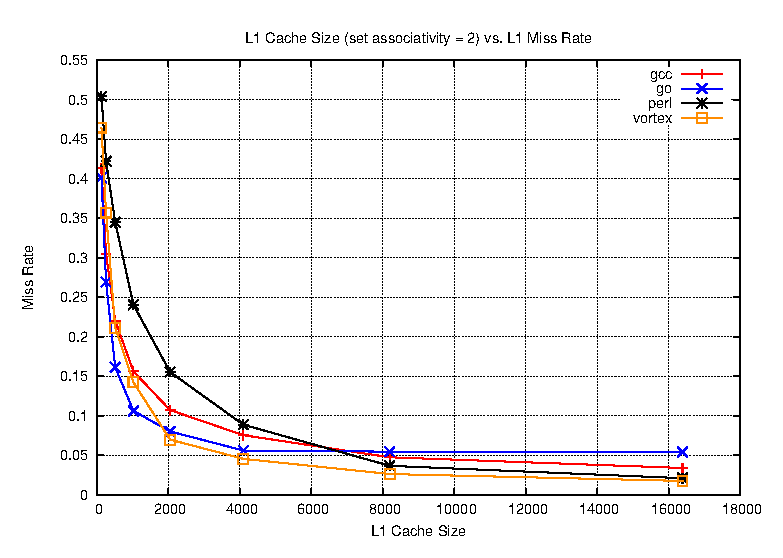
\includegraphics[scale=1.32] {l1_sa_2.eps}
    \caption{L1 Cache Size vs. L1 Miss Rate for L1 Set Associativity = 2}
    \label{fig:l1mr_graph_sa2}
\end{figure}

\begin{table}[htbp]
    \centering
    \begin{tabular}{|c|c|c|c|c|c|c|c|c|}
        \hline
        \multirow{2}[4]{*}{\bf L1 Cache Size} & \multicolumn{2}{c|}{\bf gcc} & \multicolumn{2}{c|}{\bf go} & \multicolumn{2}{c|}{\bf perl}          &\multicolumn{2}{c|}{\bf vortex}\\
        \cline{2-9} & \bf MR & \bf AAT & \bf MR & \bf AAT & \bf MR & \bf AAT & \bf MR & \bf AAT \\
        \hline
        128 & 0.4018 & 8.8393 & 0.4017 & 8.8357 & 0.4768 & 10.4126 & 0.4706 & 10.2830 \\
        256 & 0.2855 & 6.3965 & 0.1993 & 4.5857 & 0.4049 & 8.9045 & 0.3093 & 6.8967 \\
        512 & 0.2011 & 4.6255 & 0.1098 & 2.7080 & 0.3192 & 7.1065 & 0.2041 & 4.6890 \\
        1024 & 0.1427 & 3.4016 & 0.0664 & 1.7991 & 0.2345 & 5.3298 & 0.1193 & 2.9108 \\
        2048 & 0.0962 & 2.4304 & 0.0554 & 1.5727 & 0.1377 & 3.3013 & 0.0573 & 1.6131 \\
        4096 & 0.0599 & 1.6779 & 0.0542 & 1.5588 & 0.0595 & 1.6697 & 0.0313 & 1.0768 \\
        8192 & 0.0425 & 1.3309 & 0.0538 & 1.5687 & 0.0271 & 1.0086 & 0.0215 & 0.8904 \\
        16384 & 0.0283 & 1.0728 & 0.0537 & 1.6069 & 0.0177 & 0.8490 & 0.0158 & 0.8091 \\
        \hline
    \end{tabular}
    \captionsetup{justification=centering}
    \caption{Experiment Data for L1 Cache Set Associativity = 4}
    \label{tab:l1mr_data_sa4}
\end{table}

\begin{figure}
    \centering
    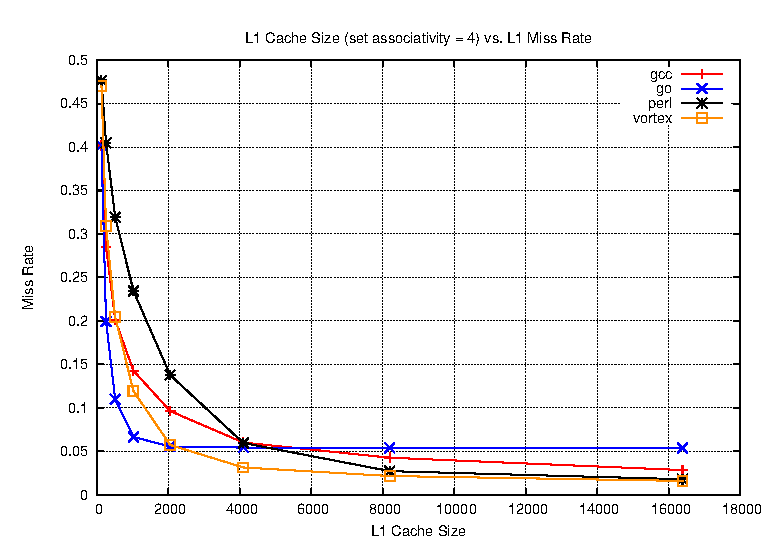
\includegraphics[scale=1.32] {l1_sa_4.eps}
    \captionsetup{justification=centering}
    \caption{L1 Cache Size vs. L1 Miss Rate for L1 Set Associativity = 4}
    \label{fig:l1mr_graph_sa4}
\end{figure}

\begin{table}[htbp]
    \centering
    \begin{tabular}{|c|c|c|c|c|c|c|c|c|}
        \hline
        \multirow{2}[4]{*}{\bf L1 Cache Size} & \multicolumn{2}{c|}{\bf gcc} & \multicolumn{2}{c|}{\bf go} & \multicolumn{2}{c|}{\bf perl}          &\multicolumn{2}{c|}{\bf vortex}\\
        \cline{2-9} & \bf MR & \bf AAT & \bf MR & \bf AAT & \bf MR & \bf AAT & \bf MR & \bf AAT \\
        \hline
        256 & 0.2795 & 6.3701 & 0.1093 & 2.7972 & 0.3989 & 8.8781 & 0.3011 & 6.8235 \\
        512 & 0.1913 & 4.5204 & 0.0846 & 2.2799 & 0.3125 & 7.0639 & 0.1780 & 4.2396 \\
        1024 & 0.1363 & 3.666 & 0.0605 & 1.7752 & 0.2290 & 5.3133 & 0.1151 & 2.9226 \\
        2048 & 0.0907 & 2.4143 & 0.0540 & 1.6433 & 0.1312 & 3.2643 & 0.0484 & 1.5253 \\
        4096 & 0.0537 & 1.6462 & 0.0538 & 1.6495 & 0.0461 & 1.4872 & 0.0290 & 1.1277 \\
        8192 & 0.0395 & 1.3694 & 0.0538 & 1.6687 & 0.0248 & 1.0605 & 0.0197 & 0.9532 \\
        16384 & 0.0277 & 1.1607 & 0.0537 & 1.7069 & 0.0168 & 0.9309 & 0.0152 & 0.8969 \\
        \hline
    \end{tabular}
    \captionsetup{justification=centering}
    \caption{Experiment Data for L1 Cache Set Associativity = 8}
    \label{tab:l1mr_data_sa8}
\end{table}

\begin{figure}
    \centering
    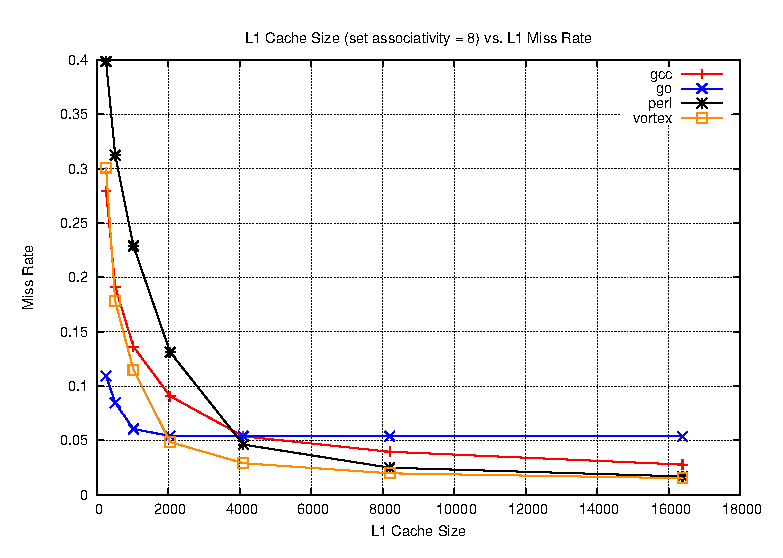
\includegraphics[scale=1.32] {l1_sa_8.eps}
    \captionsetup{justification=centering}
    \caption{L1 Cache Size vs. L1 Miss Rate for L1 Set Associativity = 8}
    \label{fig:l1mr_graph_sa8}
\end{figure}

\subsection{L1 Cache: Set Associativity and Average Access Time}
In this experiment, only L1 and L2 caches are used (victim cache is disabled). The purpose of the experiment is to study the relationship between the average access time and set associativity. The cache configuration is given in Table \ref{tab:l1aat_config}. All four traces were run with varying L1 cache set associativity. The results are tabulated in Table \ref{tab:l1aat_data}and the same is plotted as a graph in Figure \ref{fig:l1aat_graph}.

\begin{table}[htbp]
    \begin{minipage}[b]{0.45\linewidth}
        \centering
        \begin{center}
            \begin{tabular}{|l|l|}
            \hline
            \bf Cache Attributes & \bf Value \\ \hline
            Block size &  32 \\
            L1 cache size & 1024 \\
            L1 cache SA & Variable \\
            Victim cache size & Disabled \\
            L2 cache size & 4096 \\
            L2 cache SA & 4 \\
            \hline
        \end{tabular}
        \captionsetup{justification=centering}
        \captionsetup{justification=centering}
        \caption{Cache Configuration for L1 Cache Set Associativity vs. Average Access Time}
        \label{tab:l1aat_config}
    \end{center}
    \end{minipage}
    \quad
    \begin{minipage}[b]{0.45\linewidth}
        \centering
        \begin{tabular}{|c|c|c|c|c|}
            \hline
            \multirow{2}[4]{*}{\bf L1 SA} & \multicolumn{4}{c|}{\bf Average Access Time (in ns)} & 
            \cline{2-5} & \bf gcc & \bf go & \bf perl & \bf vortex \\
            \hline
            1 & 2.1047 & 2.1161 & 2.3277 & 1.4146 \\
            2 & 2.0392 & 1.7782 & 2.2431 & 1.3899 \\
            4 & 2.0517 & 1.7188 & 2.2863 & 1.3677 \\
            8 & 2.1339 & 1.7995 & 2.3503 & 1.4496 \\
            16 & 2.3143 & 2.0012 & 2.4893 & 1.6440 \\
            \hline
        \end{tabular}
        \captionsetup{justification=centering}
        \caption{Experiment Data for L1 Cache Set Associativity vs. AAT}
        \label{tab:l1aat_data}
    \end{minipage}
\end{table}


\begin{figure}
    \centering
    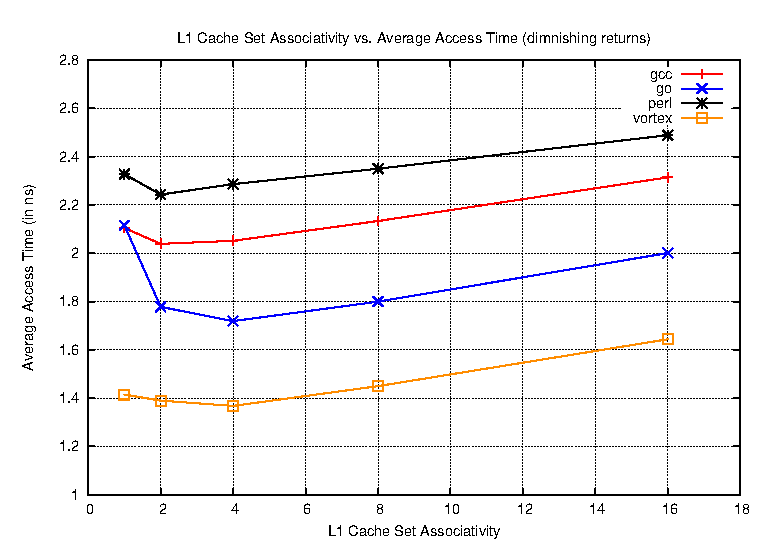
\includegraphics[scale=1.32] {l1_aat.eps}
    \captionsetup{justification=centering}
    \caption{L1 Cache Set Associativity vs. Average Access Time}
    \label{fig:l1aat_graph}
\end{figure}

\subsection{L2 Cache: Size and Miss Rate}
In this experiment, only L1 and L2 caches are used (victim cache is disabled). The purpose of the experiment is to study the relationship between the size of the L2 cache and miss rate. The cache configuration is given in Table \ref{tab:l2mr_config}. All four traces were run with fixed L1 cache size and set associativity, varying L2 cache sizes and varying L2 cache associativity. The results are tabulated in Tables \ref{tab:l2mr_data_sa1}, \ref{tab:l2mr_data_sa2}, \ref{tab:l2mr_data_sa4}, \ref{tab:l2mr_data_sa8} and the same is plotted as graphs in Figures \ref{fig:l2mr_graph_sa1}, \ref{fig:l2mr_graph_sa2}, \ref{fig:l2mr_graph_sa4}, \ref{fig:l2mr_graph_sa8}.

\begin{table}[htbp]
    \centering
    \begin{center}
        \begin{tabular}{|l|l|}
            \hline
            \bf Cache Attributes & \bf Value \\ \hline
            Block size &  32 \\
            L1 cache size & 1024 \\
            L1 cache SA & 4 \\
            Victim cache size & Disabled \\
            L2 cache size & Variable \\
            L2 cache SA & Variable \\
            \hline
        \end{tabular}
        \captionsetup{justification=centering}
        \caption{Cache Configuration for L2 Cache Size vs. Miss Rate Experiment}
        \label{tab:l2mr_config}
    \end{center}
\end{table}

\begin{table}[htbp]
    \centering
    \begin{tabular}{|c|c|c|c|c|c|c|c|c|}
        \hline
        \multirow{2}[4]{*}{\bf L2 Cache Size} & \multicolumn{2}{c|}{\bf gcc} & \multicolumn{2}{c|}{\bf go} & \multicolumn{2}{c|}{\bf perl}          &\multicolumn{2}{c|}{\bf vortex}\\
        \cline{2-9} & \bf MR & \bf AAT & \bf MR & \bf AAT & \bf MR & \bf AAT & \bf MR & \bf AAT \\
        \hline
        1024 & 0.8652 & 3.3657 & 0.9495 & 1.9000 & 0.8336 & 5.1152 & 0.7584 & 2.6132 \\
        2048 & 0.7220 & 2.9374 & 0.8766 & 1.7987 & 0.6626 & 4.2745 & 0.5888 & 2.1888 \\
        4096 & 0.5575 & 2.4457 & 0.8491 & 1.7609 & 0.4234 & 3.0987 & 0.3918 & 1.6962 \\
        8192 & 0.4083 & 2.0016 & 0.8268 & 1.7311 & 0.2691 & 2.3430 & 0.2975 & 1.4623 \\
        16384 & 0.2971 & 1.6739 & 0.8208 & 1.7253 & 0.2100 & 2.0616 & 0.2295 & 1.2967 \\
        \hline
    \end{tabular}
    \captionsetup{justification=centering}
    \caption{Experiment Data for L2 Cache Set Associativity = 1}
    \label{tab:l2mr_data_sa1}
\end{table}

\begin{figure}
    \centering
    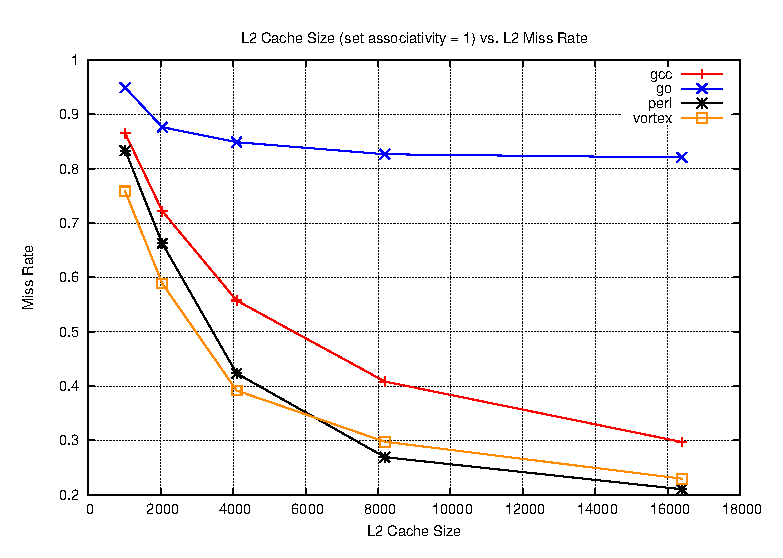
\includegraphics[scale=1.3] {l2_sa_1.eps}
    \caption{L2 Cache Size vs. L2 Cache Miss Rate for L2 Set Associativity = 1}
    \label{fig:l2mr_graph_sa1}
\end{figure}

\begin{table}[htbp]
    \centering
    \begin{tabular}{|c|c|c|c|c|c|c|c|c|}
        \hline
        \multirow{2}[4]{*}{\bf L2 Cache Size} & \multicolumn{2}{c|}{\bf gcc} & \multicolumn{2}{c|}{\bf go} & \multicolumn{2}{c|}{\bf perl}          &\multicolumn{2}{c|}{\bf vortex}\\
        \cline{2-9} & \bf MR & \bf AAT & \bf MR & \bf AAT & \bf MR & \bf AAT & \bf MR & \bf AAT \\
        \hline
        1024 & 0.8582 & 3.3485 & 0.9205 & 1.8611 & 0.8520 & 5.2118 & 0.7706 & 2.6469 \\
        2048 & 0.6708 & 2.7874 & 0.8720 & 1.7938 & 0.6202 & 4.0716 & 0.4777 & 1.9133 \\
        4096 & 0.4926 & 2.2550 & 0.8220 & 1.7248 & 0.3594 & 2.7893 & 0.3169 & 1.5115 \\
        8192 & 0.3254 & 1.7565 & 0.8156 & 1.7172 & 0.1562 & 1.7932 & 0.2000 & 1.2211 \\
        16384 & 0.2359 & 1.4939 & 0.8104 & 1.7125 & 0.0884 & 1.4685 & 0.1451 & 1.0880 \\
        \hline
    \end{tabular}
    \captionsetup{justification=centering}
    \caption{Experiment Data for L2 Cache Set Associativity = 2}
    \label{tab:l2mr_data_sa2}
\end{table}

\begin{figure}
    \centering
    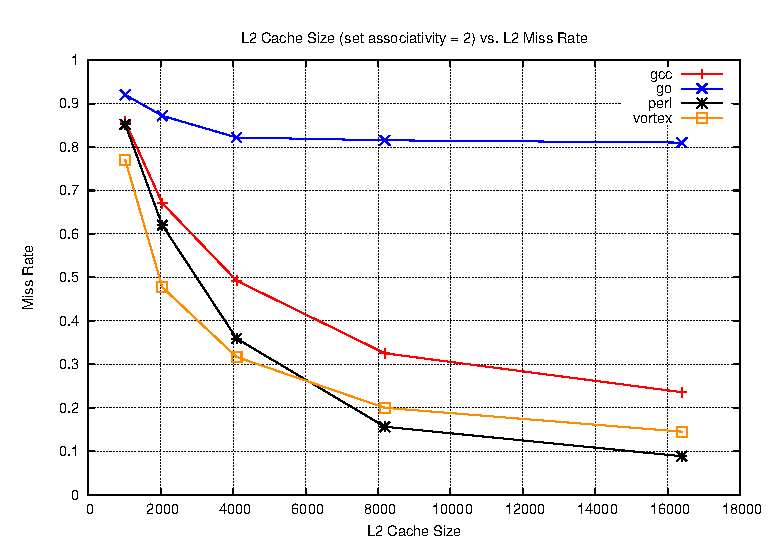
\includegraphics[scale=1.3] {l2_sa_2.eps}
    \caption{L2 Cache Size vs. L2 Cache Miss Rate for L2 Set Associativity = 2}
    \label{fig:l2mr_graph_sa2}
\end{figure}

%\clearpage

\begin{table}[htbp]
    \centering
    \begin{tabular}{|c|c|c|c|c|c|c|c|c|}
        \hline
        \multirow{2}[4]{*}{\bf L2 Cache Size} & \multicolumn{2}{c|}{\bf gcc} & \multicolumn{2}{c|}{\bf go} & \multicolumn{2}{c|}{\bf perl}          &\multicolumn{2}{c|}{\bf vortex}\\
        \cline{2-9} & \bf MR & \bf AAT & \bf MR & \bf AAT & \bf MR & \bf AAT & \bf MR & \bf AAT \\
        \hline
        1024 & 0.8632 & 3.3705 & 0.9090 & 1.8485 & 0.8871 & 5.3963 & 0.7835 & 2.6850 \\
        2048 & 0.6590 & 2.7593 & 0.8308 & 1.7398 & 0.5759 & 3.8649 & 0.4384 & 1.8210 \\
        4096 & 0.4224 & 2.0517 & 0.8153 & 1.7188 & 0.2549 & 2.2863 & 0.2571 & 1.3677 \\
        8192 & 0.2984 & 1.6828 & 0.8104 & 1.7132 & 0.1161 & 1.6074 & 0.1742 & 1.1624 \\
        16384 & 0.1985 & 1.3891 & 0.8096 & 1.7148 & 0.0754 & 1.4160 & 0.1316 & 1.0601 \\
        \hline
    \end{tabular}
    \captionsetup{justification=centering}
    \caption{Experiment Data for L2 Cache Set Associativity = 4}
    \label{tab:l2mr_data_sa4}
\end{table}

\begin{figure}
    \centering
    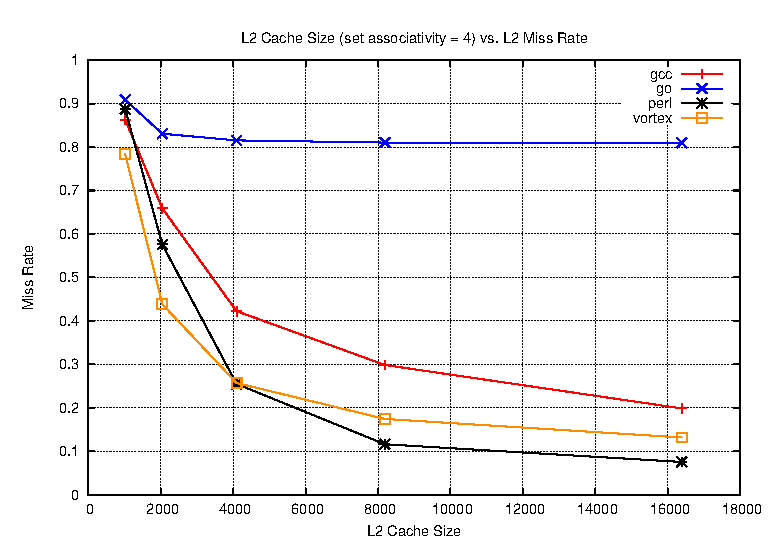
\includegraphics[scale=1.3] {l2_sa_4.eps}
    \captionsetup{justification=centering}
    \caption{L2 Cache Size vs. L2 Cache Miss Rate for L2 Set Associativity = 4}
    \label{fig:l2mr_graph_sa4}
\end{figure}

\begin{table}[htbp]
    \centering
    \begin{tabular}{|c|c|c|c|c|c|c|c|c|}
        \hline
        \multirow{2}[4]{*}{\bf L2 Cache Size} & \multicolumn{2}{c|}{\bf gcc} & \multicolumn{2}{c|}{\bf go} & \multicolumn{2}{c|}{\bf perl}          &\multicolumn{2}{c|}{\bf vortex}\\
        \cline{2-9} & \bf MR & \bf AAT & \bf MR & \bf AAT & \bf MR & \bf AAT & \bf MR & \bf AAT \\
        \hline
        1024 & 0.7987 & 3.1916 & 0.8700 & 1.8007 & 0.8230 & 5.1044 & 0.6761 & 2.4279 \\
        2048 & 0.6297 & 2.6858 & 0.8200 & 1.7313 & 0.5631 & 3.8254 & 0.4036 & 1.7456 \\
        4096 & 0.3762 & 1.9274 & 0.8113 & 1.7198 & 0.1975 & 2.0269 & 0.2418 & 1.3412 \\
        8192 & 0.2777 & 1.6351 & 0.8102 & 1.7196 & 0.1060 & 1.5808 & 0.1652	& 1.1516 \\
        16384 & 0.1941 & 1.3902 & 0.8096 & 1.7214 & 0.0717 & 1.4214 & 0.1271 & 1.0609 \\
        \hline
    \end{tabular}
    \captionsetup{justification=centering}
    \caption{Experiment Data for L2 Cache Set Associativity = 8}
    \label{tab:l2mr_data_sa8}
\end{table}

\begin{figure}
    \centering
    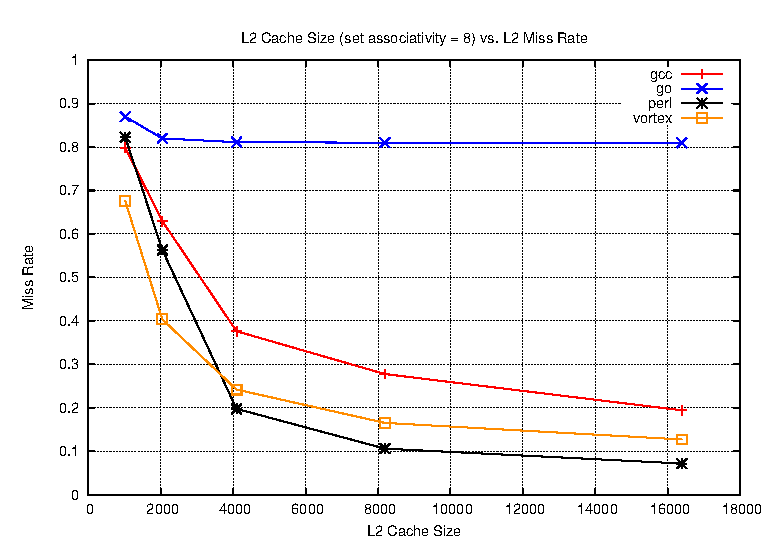
\includegraphics[width=\textwidth] {l2_sa_8.eps}
    \captionsetup{justification=centering}
    \caption{L2 Cache Size vs. L2 Cache Miss Rate for L2 Set Associativity = 8}
    \label{fig:l2mr_graph_sa8}
\end{figure}

%\clearpage

\subsection{Victim Cache: Size and Miss Rate}
In this experiment, all three caches (L1, victim and L2) are used. The purpose of the experiment is to study the relationship between the size of the victim cache and how it affects the miss rates of L1 and L2 caches. The cache configuration is given in Table \ref{tab:vcmr_config}. All four traces were run with fixed L1 and L2 cache sizes and set associativity and by varying the victim cache size. The result is tabulated in Table \ref{tab:vcmr_data}, and the same is plotted as a graph in Figure \ref{fig:vcmr_graph}.

\begin{table}[htbp]
    \centering
    \begin{center}
        \begin{tabular}{|l|l|}
            \hline
            \bf Cache Attributes & \bf Value \\ \hline
            Block size &  64 \\
            L1 cache size & 8192 \\
            L1 cache SA & 2 \\
            Victim cache size & Variable \\
            L2 cache size & 16384  \\
            L2 cache SA & 4 \\
            \hline
        \end{tabular}
        \captionsetup{justification=centering}
        \caption{Cache Configuration for Victim Cache Size vs. L1/L2 Cache Miss Rate Experiment}
        \label{tab:vcmr_config}
    \end{center}
\end{table}

\begin{table}[htbp]
    \centering
    \begin{tabular}{|c|c|c|c|c|c|c|c|c|}
        \hline
        \multirow{2}[4]{*}{\bf Victim Cache Size} & \multicolumn{2}{c|}{\bf gcc} & \multicolumn{2}{c|}{\bf go} & \multicolumn{2}{c|}{\bf perl} &\multicolumn{2}{c|}{\bf vortex}\\
        \cline{2-9} & \bf MR_{L1} & \bf MR_{L2} & \bf MR_{L1} & \bf MR_{L2} & \bf MR_{L1} & \bf MR_{L2} & \bf MR_{L1} & \bf MR_{L2} \\
        \hline
        128 & 0.0416 & 0.4922 & 0.0291 & 0.9877 & 0.0339 & 0.3943 & 0.0217 & 0.5475 \\
        512 &  0.0352 & 0.5723 & 0.0288 & 1.0000 & 0.0281 & 0.4678 & 0.0180 & 0.6493 \\
        1024 & 0.0309 & 0.6320 & 0.0288 & 1.0000 & 0.0250 & 0.5080 & 0.0163 & 0.7023 \\
        2048 & 0.0262 & 0.7144 & 0.0287 & 1.0000 & 0.0204 & 0.5690 & 0.0146 & 0.7754 \\
        4096 & 0.0228 & 0.7480 & 0.0287 & 1.0000 & 0.0147 & 0.7154 & 0.0126 & 0.8585 \\
        \hline
    \end{tabular}
    \captionsetup{justification=centering}
    \caption{Experiment Data for Victim Cache Size vs. L1/L2 Caches Miss Rate}
    \label{tab:vcmr_data}
\end{table}

\begin{figure}
    \centering
    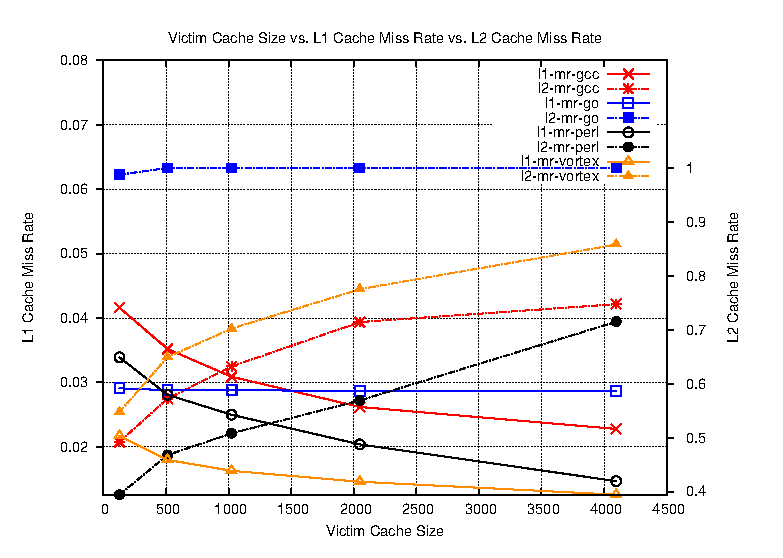
\includegraphics[scale=1.32] {vc_l1l2_mr.eps}
    %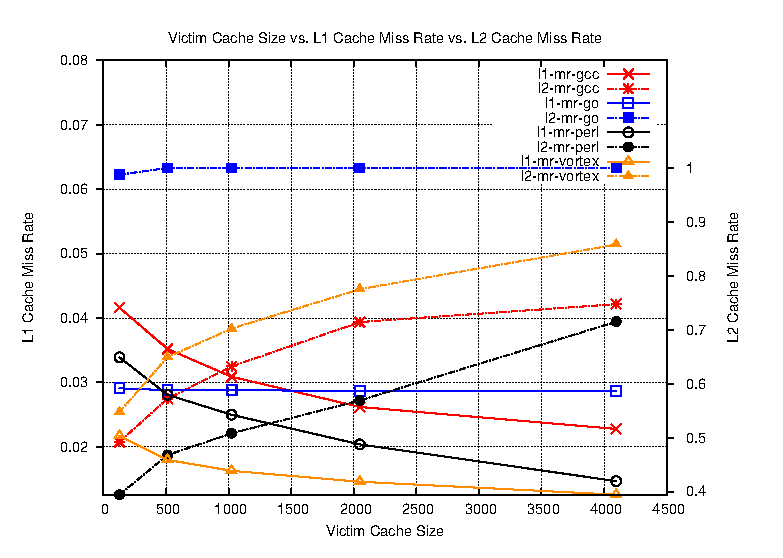
\includegraphics[width=\textwidth] {vc_l1l2_mr.eps}
    \captionsetup{justification=centering}
    \caption{Victim Cache Size vs. L1 \& L2 Caches Miss Rate}
    \label{fig:vcmr_graph}
\end{figure}

\begin{figure}
    \centering
    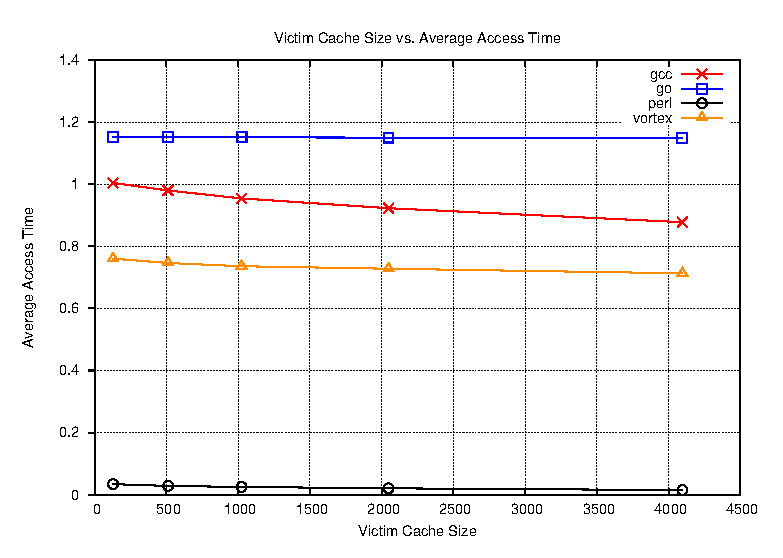
\includegraphics[scale=1.32] {vc_aat.eps}
    %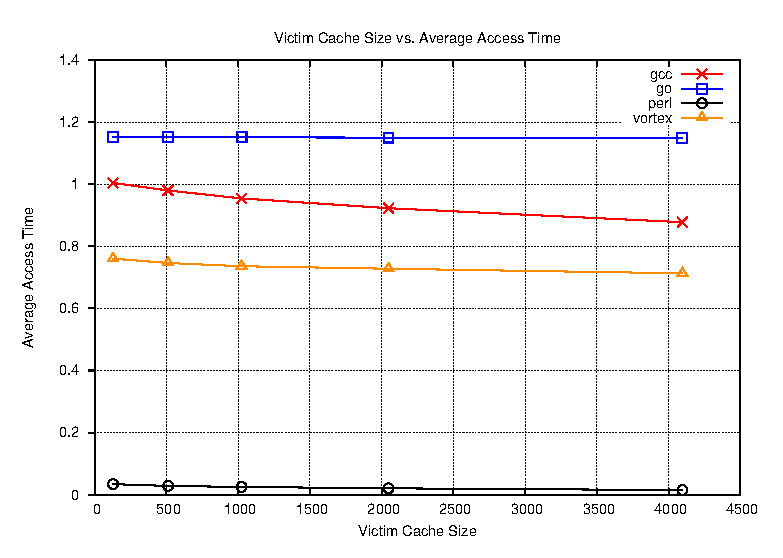
\includegraphics[width=\textwidth] {vc_aat.eps}
    \captionsetup{justification=centering}
    \caption{Victim Cache Size vs. Average Access Time}
    \label{fig:vcaat_graph}
\end{figure}

\section{Cache Performance Analysis}
A cache's performance can be affected by many factors such as cache parameters (block size, capacity, set associativity, replacement algorithms and so on), other caches (victim and other lower level caches) in the cache pipeline and their parameters and instruction/data access patterns (data exhibiting spatial vs. temporal locality). Only cache attributes can be fine tuned by computer architects to improve the performance of the caches as locality and data access patterns are controlled by programmers and compilers. Two main calculations help us in determining a cache's performance: cache average access time and cache miss rate. The former is dependant of the latter.

The cache performance can be improved in three ways:
\begin{enumerate}
    \item Reduce miss rate
    \begin{enumerate}
        \item Modify block size, cache size, associativity
        \item Enable hardware and software prefetching
        \item Optimize data and instructions layout
    \end{enumerate}
    \item Reduce miss penalty
    \begin{enumerate}
        \item Employ victim and L2 caches
        \item Employ write buffers
        \item Enable early restart
        \item Fetch critical word first
    \end{enumerate}
    \item Reduce hit time
    \begin{enumerate}
        \item TLB and L1 cache access in parallel
        \item Pipeline writes
    \end{enumerate}
\end{enumerate}

The cache simulator that was built as part of this project can be used to analyze and evaluate cache performance by varying the cache attributes such as block size, cache size, associativity. Brief description on how the cache performance is affected on changing the cache attributes is given in Table \ref{tab:perf_metrics}.

\begin{table}[h!]
    \centering
    \begin{center}
        \begin{tabular}{|p{3cm}|p{6cm}|p{6cm}|}
            \hline
            \bf Affected Cache Attribute & \bf Advantages & \bf Disadvantages \\ \hline
            Block size &  Increasing it reduces the miss rate by exploiting spatial locality of the data & Increases cache pollution and miss penalty in case of cache misses \\ \hline
            Cache size & Increasing it makes more data available in caches and thus reduces the miss rate & Increases hit time (search takes more time) and increases space requirements on chip \\ \hline
            Set associativity & Increasing it reduces conflict misses and thus reduces miss rate & Increases the hit time for the same cache size and increases power consumption \\ \hline
        \end{tabular}
        \captionsetup{justification=centering}
        \caption{Cache Performance Tuning}
        \label{tab:perf_metrics}
    \end{center}
\end{table}

\subsection{Trends}
\subsubsection{Cache Size}
It can be inferred from the graphs for L1 cache sizes vs. miss rate (in Figures \ref{fig:l1mr_graph_sa1}, \ref{fig:l1mr_graph_sa2}, \ref{fig:l1mr_graph_sa4}, \ref{fig:l1mr_graph_sa8}) and from the graphs for L2 cache sizes vs. miss rate (in Figures \ref{fig:l2mr_graph_sa1}, \ref{fig:l2mr_graph_sa2}, \ref{fig:l2mr_graph_sa4}, \ref{fig:l2mr_graph_sa8}) that increasing the cache size improves the cache performance by reducing the miss rate. 

Also, increasing the cache size alone is not sufficient enough to reduce the miss rate: data access pattern also plays an important role. Sparsely distributed data pollutes the cache and reduces the hit rate. This can be clearly seen in Figures \ref{fig:l2mr_graph_sa2}, \ref{fig:l2mr_graph_sa4} and \ref{fig:l2mr_graph_sa8} for trace ``go". The miss rate doesn't decrease greatly as the cache size is increased. This could be attributed to the fact that the ``go" trace file has sparse data accesses.

\subsubsection{Set Associativity}
``The law of negative returns" can be clearly seen in Figure \ref{fig:l1aat_graph} where increasing the set associativity of a cache beyond a certain point, actually increases the overall average access time. This supports the fact that a set associativity of more than 4 is not required in most cases and it also reiterates that data access patterns are as important as cache attributes when it comes to optimal cache performance.

\subsubsection{Victim Cache}
Victim caches usually complement L1 caches. They are fully associative, but smaller than L1 caches. Contents of L1 and victim caches are mutually exclusive, thus no part of cache memory is used in storing redundant data. Once enabled, they greatly reduce the miss rate and miss penalty of L1 cache. Thus, the performance of L1 cache will be improved in a significant manner in the presence of a victim cache. This could be seen in Figure \ref{fig:vcmr_graph} where L1 cache miss rate reduces as the size of victim cache is increased. 

But, victim caches affects the performance of L2 caches. To put it more clearly, victim caches enhances the performance of L1 caches by degrading the performance of L2 caches. This could be again seen in Figure \ref{fig:vcmr_graph} where the miss rate of L2 cache increases as the size of victim cache is increased.

\subsection{Best Memory Hierarchy Configuration}
The experiment data in this report provides clear insight on cache performance. Two major attributes determines the cache performance: miss rate and average access time. The following three points are based on the experiment data:
\begin{enumerate}
\item The miss rate of a cache decreases as cache size increases.
\item The average access time decreases as more caches are added to the pipeline (victim and L2).
\item The data access pattern also plays a huge role. The same cache performs much better for access patterns following a locality model (vortex\_trace) as opposed to a sparse access trace (go\_trace).
\end{enumerate}

The best cache configuration is given in Table \ref{tab:best_cache_config}.
\begin{table}[htbp]
    \centering
    \begin{center}
        \begin{tabular}{|l|l|}
            \hline
            \bf Cache Attributes & \bf Value \\ \hline
            Block size &  64 \\
            L1 cache size & 4096 \\
            L1 cache SA & 2 \\
            Victim cache size & 1024 \\
            L2 cache size & 16384  \\
            L2 cache SA & 4 \\ \hline
            L1 miss rate & 0.0172 \\
            L2 miss rate & 0.6268 \\
            Average Access Time & 0.7790 ns \\
            \hline
        \end{tabular}
        \captionsetup{justification=centering}
        \caption{Best Memory Hierarchy Cache Configuration}
        \label{tab:best_cache_config}
    \end{center}
\end{table}

\subsection{Benchmarks Comparison}
All the experiments were run using four memory trace benchmarks - gcc, go, perl and vortex, each with a different type of memory access pattern. It is evident from the plots and tables presented above that vortex trace has the optimal memory access pattern that makes best use of cache hierarchy. Perl trace performs slightly better than vortex when L2 cache is present. Of all four, go trace has the most cache unfriendly access patterns. It has the highest miss rate and average access time, which does not imporve even on enabling victim and L2 caches (refer \ref{fig:vcmr_graph}).

A key insight to be learned: cache parameters alone cannot ensure optimal cache performance; it also depends on the data access patterns of a running program. As famously put by Herb Sutter, "The free lunch is over" for software programmers. Application and system engineers should include necessary optimizations in code to make the best use of the hierarchical memory system.

\section{Conclusion}
The key takeaway of this project and the project report is the understanding of various cache attributes and how it affects the performance of a cache (in both positive and negative way). The experiments and the assoiciated plots shows that cache size, additional caches and data access pattern plays a huge role in cache performance tuning along with other parameters such as block size and set assoiciativity. 

\end{document}
